\section{Experiments}
\subsection{Experimental Settings}


\paragraph{Datasets} We train our model on datasets DL3DV \cite{ling2024dl3dv} and RealEstate10K \cite{zhou2018stereo}, which contains in-door and out-door scene. We test in the remained set from training of DL3DV and RealEstate10K, and test the out-of-domain performance on DTU \cite{jensen2014large}.

\newcommand{\w}[1]{\text{w/\ #1}}
\newcommand{\wo}[1]{\text{w/o\ #1}}


\newcommand{\cmark}{\ding{51}} % ✓
\newcommand{\xmark}{\ding{55}} % ✗
\newcolumntype{Y}{>{\centering\arraybackslash}m{2.2cm}}
% 窄中心列类型
\newcolumntype{C}[1]{>{\centering\arraybackslash}m{#1}}
% 自适应文本列
%\newcolumntype{Y}{>{\raggedright\arraybackslash}X}
\newcolumntype{Y}{>{\raggedright\arraybackslash}p{1.8cm}}


\begin{table*}[htbp]
\centering
\caption{\textbf{Novel view synthesis performance comparison on the RealEstate10K with 2 views as input}. 
Our method largely outperforms pose-free and pose-required methods across all overlap settings, especially for small overlap setting.
The \textbf{best} and \underline{second-best} results are highlighted.}
\label{tab:re10k_nvs}
%\setlength{\tabcolsep}{6.5pt}
\renewcommand{\arraystretch}{1.25}
\scriptsize
\resizebox{\linewidth}{!}{%
\begin{tabular}{l l ccc ccc ccc ccc}
\toprule
& \multirow{2}{*}{\textbf{Method}} &
\multicolumn{3}{c}{\textbf{Small}} &
\multicolumn{3}{c}{\textbf{Medium}} &
\multicolumn{3}{c}{\textbf{Large}} &
\multicolumn{3}{c}{\textbf{Average}} \\
\cmidrule(lr){3-5}\cmidrule(lr){6-8}\cmidrule(lr){9-11}\cmidrule(lr){12-14}
& & PSNR$\uparrow$ & SSIM$\uparrow$ & LPIPS$\downarrow$ &
PSNR$\uparrow$ & SSIM$\uparrow$ & LPIPS$\downarrow$ &
PSNR$\uparrow$ & SSIM$\uparrow$ & LPIPS$\downarrow$ &
PSNR$\uparrow$ & SSIM$\uparrow$ & LPIPS$\downarrow$ \\
\midrule
\multirow{4}{*}{\rotatebox{90}{Pose-Required}} 
& pixelNeRF \cite{yu2021pixelnerf} & 18.417 & 0.601 & 0.526 & 19.930 & 0.632 & 0.480 & 20.869 & 0.639 & 0.458 & 19.824 & 0.626 & 0.485 \\
& AttnRend \cite{du2023learning} & 19.151 & 0.663 & 0.368 & 22.532 & 0.763 & 0.269 & 25.897 & 0.845 & 0.186 & 22.664 & 0.762 & 0.269 \\
& pixelSplat \cite{charatan2024pixelsplat} & 20.263 & 0.717 & 0.266 & 23.711 & 0.809 & 0.181 & 27.151 & 0.879 & 0.122 & 23.848 & 0.806 & 0.185 \\
& MVSplat \cite{chen2024mvsplat}   & 20.353 & 0.724 & 0.250 & 23.778 & 0.812 & 0.173 & 27.408 & 0.884 & 0.116 & 23.977 & 0.811 & 0.176 \\
\midrule
\multirow{9}{*}{\rotatebox{90}{Pose-Free}} 
& DUST3R \cite{wang2024dust3r}  & 14.101 & 0.432 & 0.468 & 15.419 & 0.451 & 0.432 & 16.427 & 0.453 & 0.402 & 15.382 & 0.447 & 0.432 \\
& MAST3R \cite{leroy2024grounding}   & 13.534 & 0.407 & 0.494 & 14.945 & 0.436 & 0.451 & 16.028 & 0.444 & 0.418 & 14.907 & 0.431 & 0.452 \\
& Splatt3r \cite{smart2024splatt3r}  & 14.352 & 0.475 & 0.472 & 15.529 & 0.502 & 0.425 & 15.817 & 0.483 & 0.421 & 15.318 & 0.490 & 0.436 \\
& CoPoNeRF \cite{hong2023unifying} & 17.393 & 0.585 & 0.462 & 18.813 & 0.616 & 0.392 & 20.464 & 0.652 & 0.318 & 18.938 & 0.619 & 0.388 \\
& NopoSplat \cite{ye2024no} & 22.514 & 0.784 & 0.210 & 24.899 & 0.839 & 0.160 & 27.411 & 0.883 & 0.119 & 25.033 & 0.838 & 0.160 \\
& FLARE \cite{zhang2025flare}  &  22.468 & 0.763 & 0.198 & 24.872 & 0.836 & 0.162 & 27.012 & 0.881 & 0.123 & 24.891 & 0.831 & 0.161  \\ 
& AnySplat \cite{jiang2025anysplat} &  22.703	& 0.781	& 0.221 &	25.107	& 0.844 &	0.156	& 27.414	& 0.883	& 0.118 & 25.176 & 0.839 & 0.161 \\ 
\cmidrule(lr){2-14}
& \textbf{IFSplat(Ours)} & \underline{24.207} & \underline{0.813} & \underline{0.183} & \underline{26.421} & \underline{0.853} & \underline{0.145} & \underline{27.895} & \underline{0.891} & \underline{0.114} & \underline{26.291} & \underline{0.854} & \underline{0.145} \\
& \textbf{GIFSplat(Ours)} & \textbf{24.617} & \textbf{0.827} & \textbf{0.181} & \textbf{26.714} & \textbf{0.866} & \textbf{0.131} & \textbf{27.987} & \textbf{0.902} & \textbf{0.112} & \textbf{26.559}  & \textbf{0.867} & \textbf{0.138} \\
\bottomrule
\end{tabular}}
\end{table*}



% \begin{figure*}[htbp]
%   \centering
%   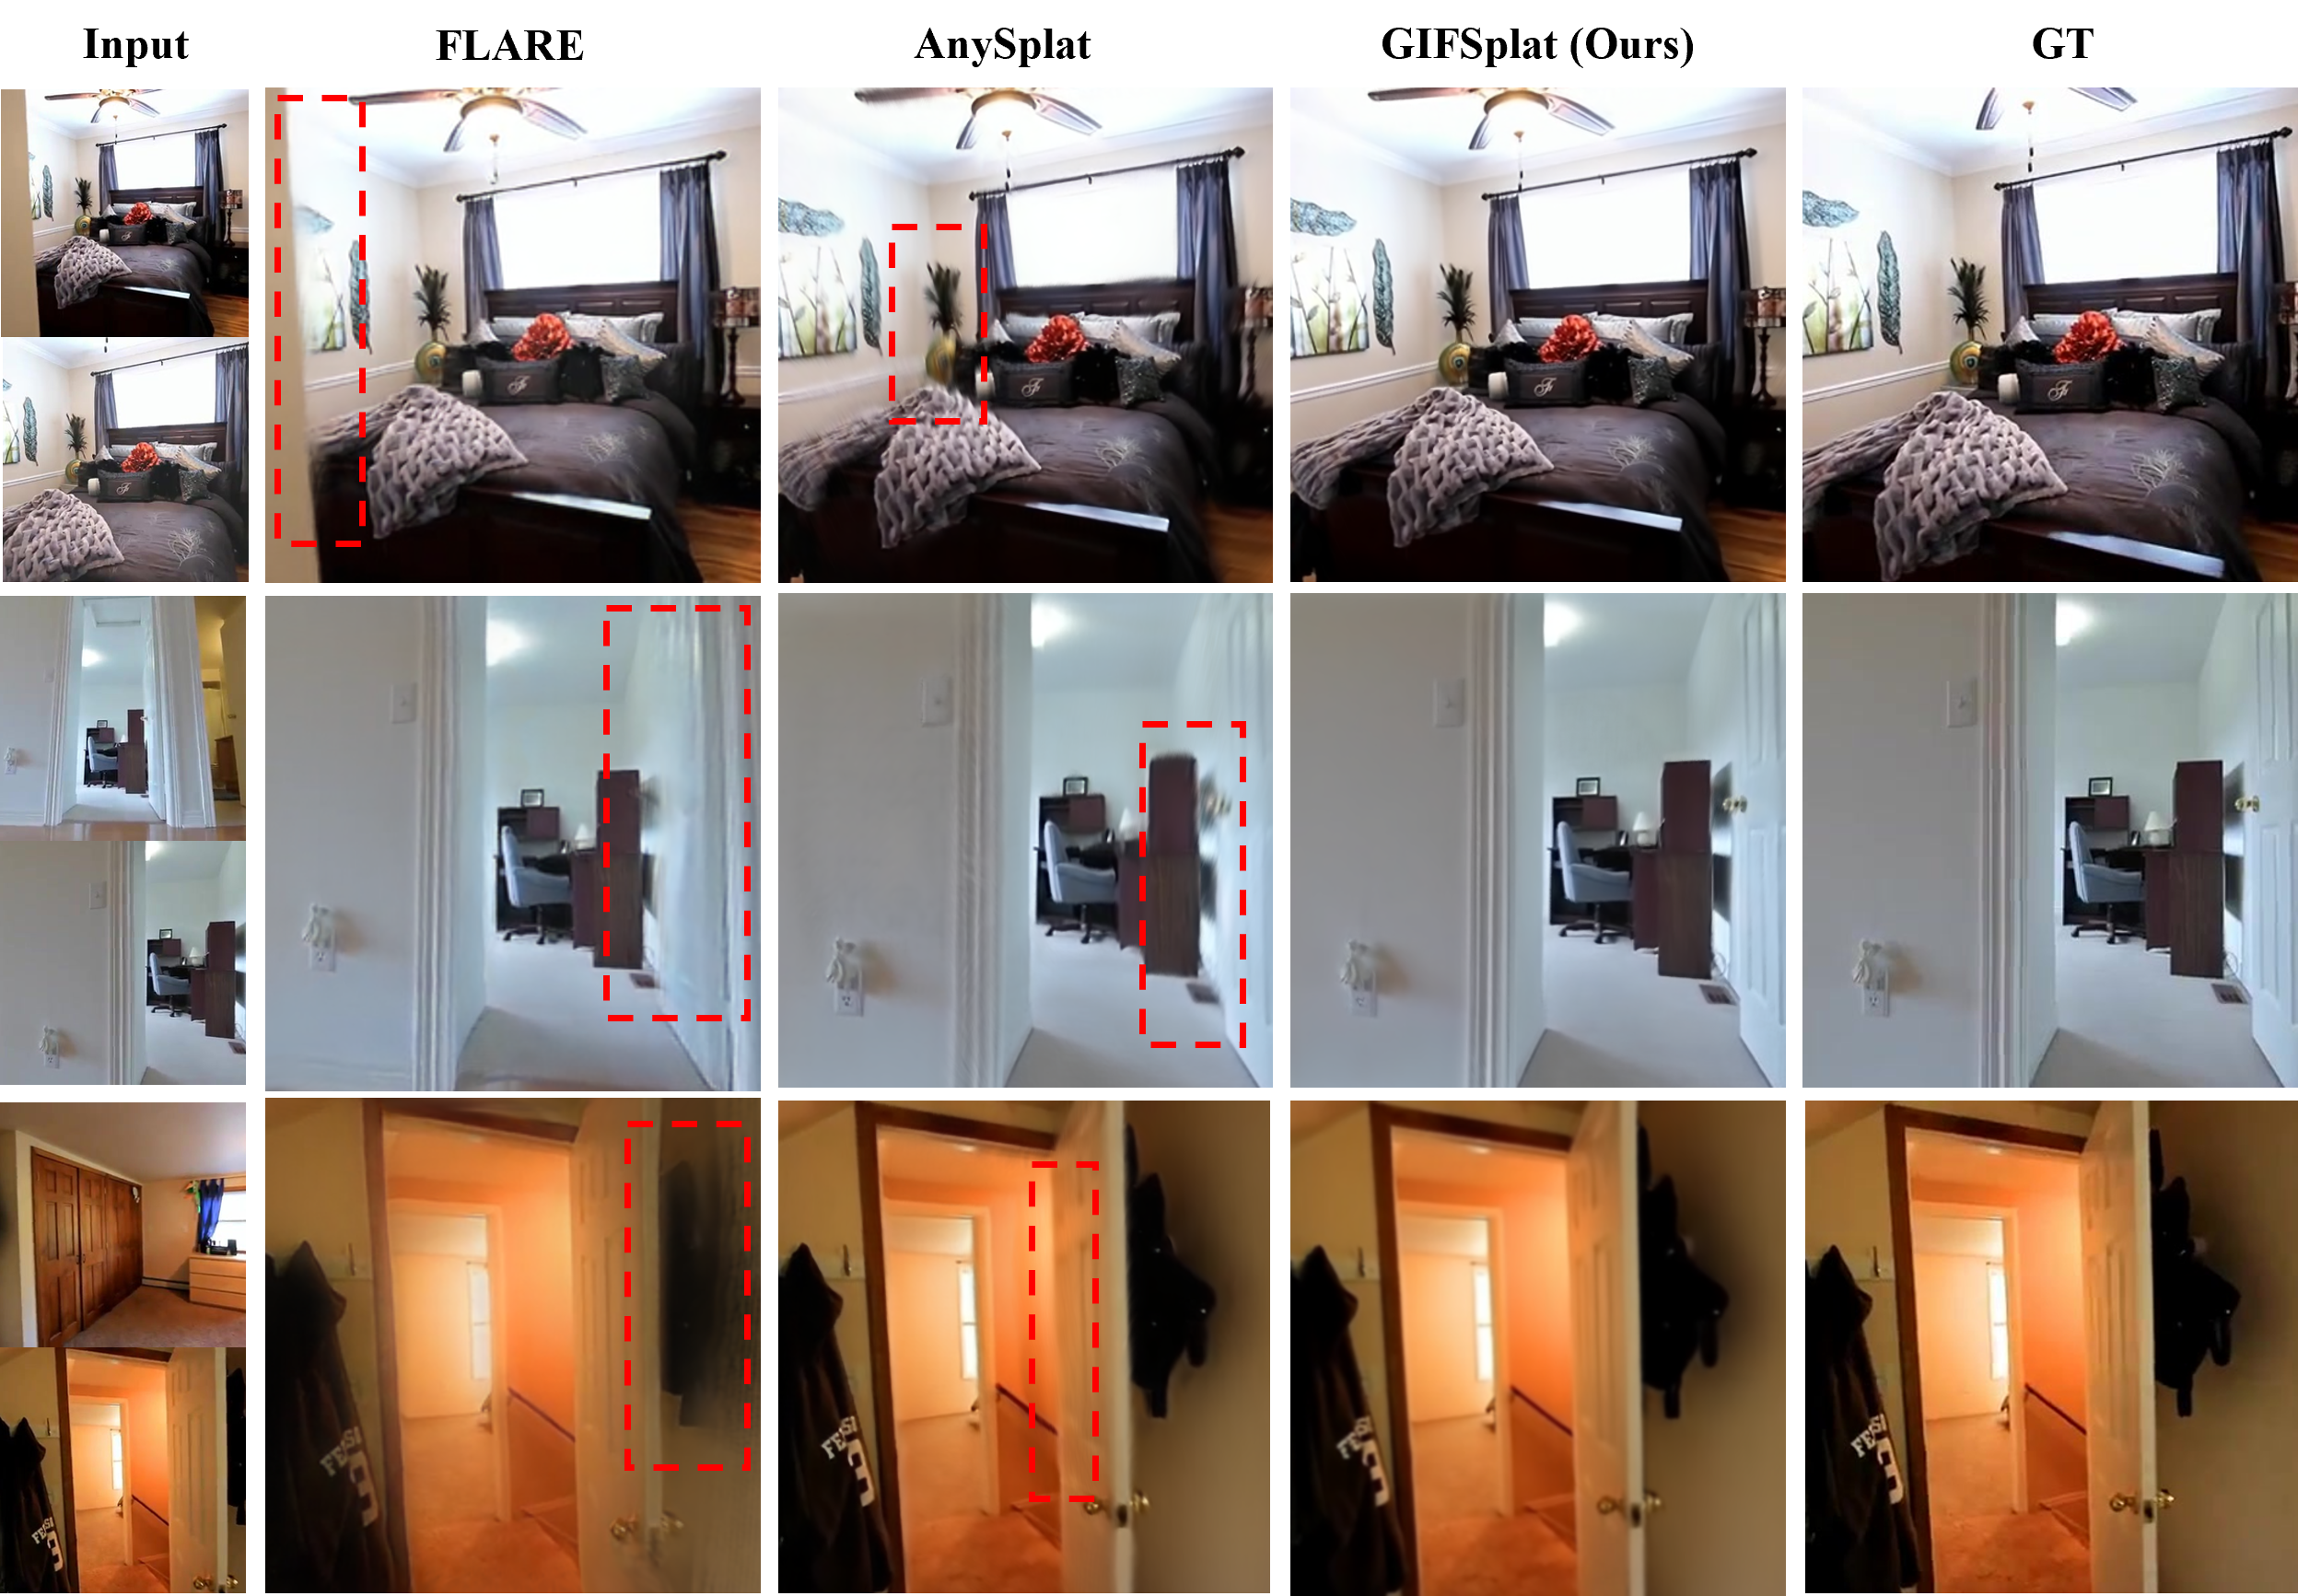
\includegraphics[width=\linewidth]{pics/Real10K.png}
%   \caption{\textbf{Qualitative comparisons} on representative indoor scenes RealEstate10K. 
% From left to right: inputs, FlARE, Anysplat, initial stage of our method , our iterative residual model IFSplat, our GIFSplat with generative prior, and GT. 
% \textbf{GIFSplat} produces crisper boundaries (e.g., door frames, wall corners) and richer textures, while suppressing texture sticking, blur at disocclusions, and floaters under large viewpoint changes. }
% \label{fig:visual}
% \end{figure*}

\begin{figure*}[ht]
  \centering
  % 在双栏模板中，单栏宽度用 \columnwidth
  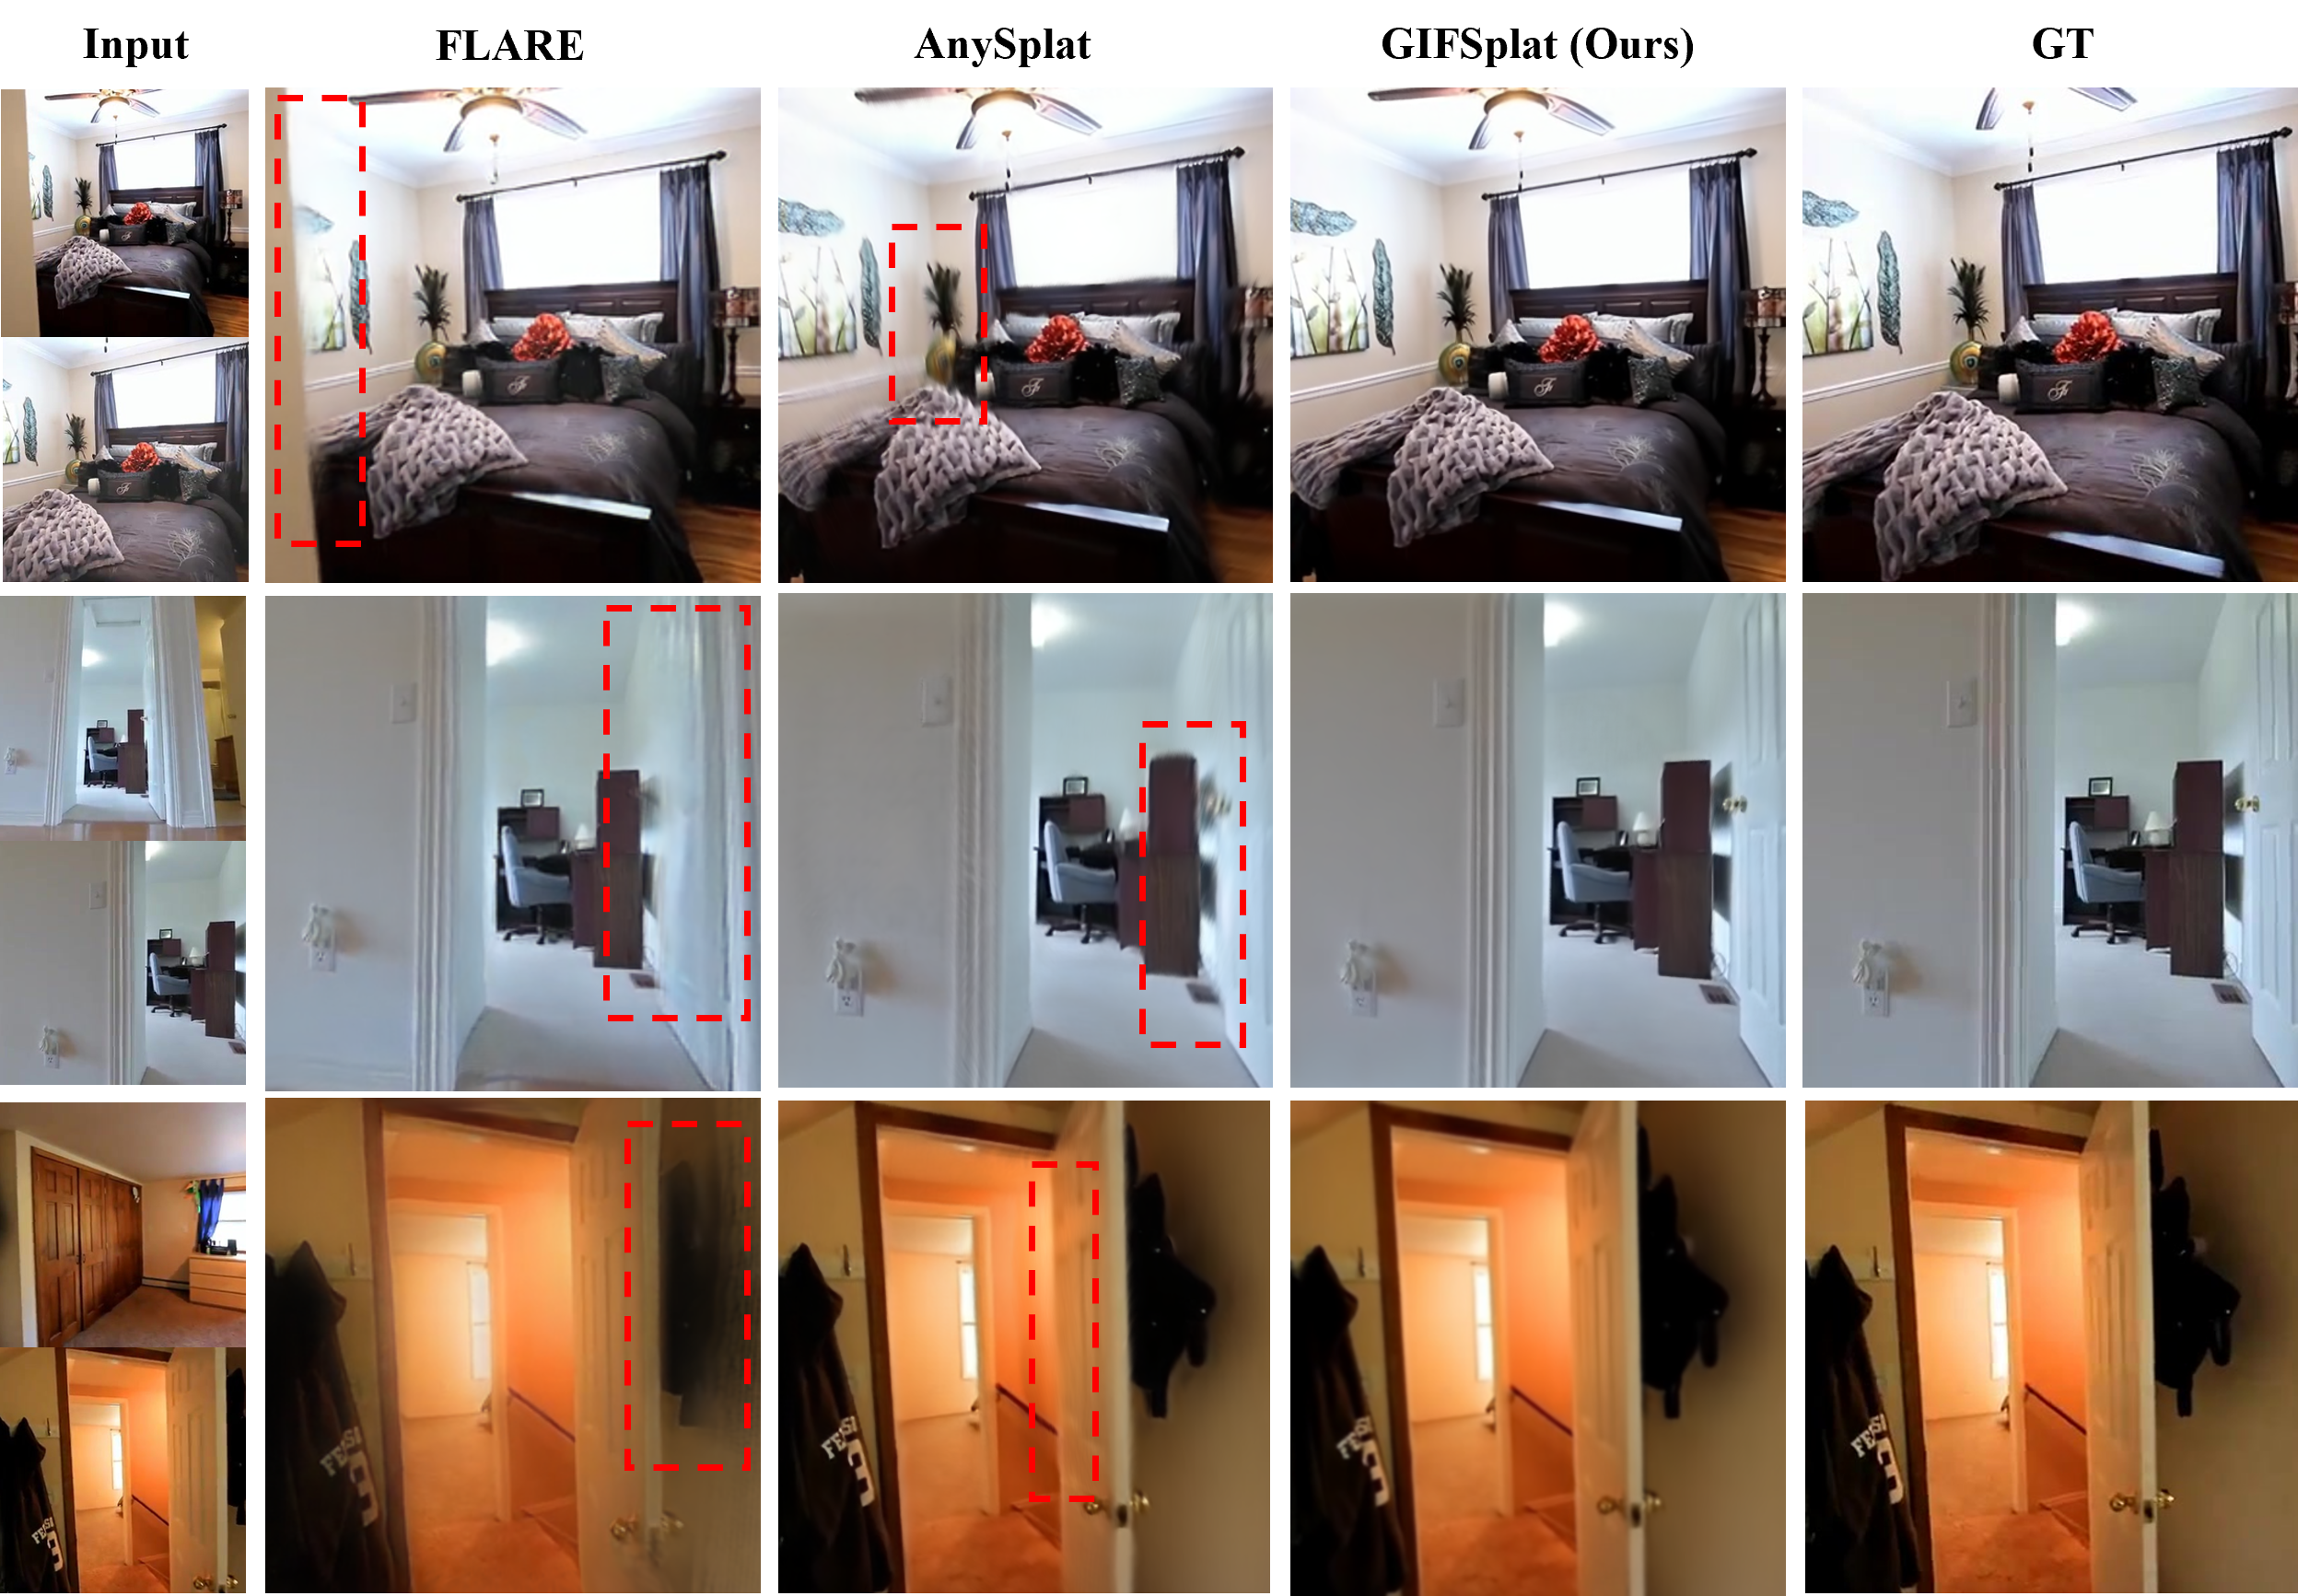
\includegraphics[width=0.97\linewidth]{pics/Real10K.png}
  \caption{\textbf{Qualitative comparisons on representative indoor scenes from RealEstate10K.}
 Columns: sparse input views, FLARE, AnySplat, our GIFSplat with generative prior, and ground truth (GT). Red dashed boxes highlight that GIFSplat recovers sharper boundaries (e.g., door frames, wall corners), more faithful textures, and fewer artifacts such as texture sticking.}
  \label{fig:re10k}
\end{figure*}

% \begin{figure}[t]
%   \centering
%   % 在双栏模板中，单栏宽度用 \columnwidth
%   \includegraphics[width=\linewidth]{pics/Real10K_2.png}
%   \caption{.}
%   \label{fig:single}
% \end{figure}


\paragraph{Baselines and metrics} 
To compare with previous methods, we mainly consider three evaluation setups. First, novel view synthesis from 8 input views at 448×448 resolution on DL3DV, where we adopt PixelSplat, MVSplat, FLARE, AnySplat as baselines. Second, we also evaluate on the commonly used 2-view at 256×256 resolution setup on RealEstate10K \cite{zhou2018stereo} with different overlap settings, except for aforementioned baseline, we compare with benchmark in ~\cite{ye2024no}. In addition, we test the generalization ability on DTU using model trained on RealEstate10K. We use PSNR, SSIM, LPIPS as our metric to evaluate the performance of novel view synthesis. More information is provided in the  Appendix.



\paragraph{Experimental settings} We use gsplat \cite{yu2024mip} as differential rasterizer and AdamW as optimizer . We train and evaluate our model on 4 NVIDIA DGX H200 141GB GPU for all experiments. For experiments on DL3DV, we fine-tuned the initializer for 30K steps and trained the iterative gaussians head for 300K steps. For experiments on RealEstate10K, we fine-tuned the initializer for 50K steps and trained the iterative gaussians head for 100K steps. More information is provided in the Appendix. For DL3DV, we follow the FLARE test split and evaluate in 112 unseen scenes (8 views for input, 9 views for evaluation). For RealEstate10K (2 views for input, 3 views for evaluation) and generalization on DTU (2 views for input, 4 views for evaluation) experiments, we all follow the NopoSplat evaluation setting. 


\subsection{Comparison with Feed-forward baseline}

\paragraph{2-view evaluation on RealEstate10K}

~\cref{tab:re10k_nvs} and ~\cref{fig:re10k} show the quantitative and qualitative results, respectively. We follow the settings of NopoSplat \cite{ye2024no}, splitting the scene to three parts according to the overlap ratio. Across all setting, our iterative residual model IFSplat get the better results than existing baselines. Moreover, GIFSplat gets the best results with the help of generative prior, preserving fine textures, with fewer blurs than all other models. Notably, some implausible deformation such as the door and wardrobe are rectified by generative prior. %A few forward-only refinement steps progressively repair disocclusion edges and small holes, while generative prior mitigates over-smoothing in sparsely observed regions. Overall, GIFSplat yields cleaner, more complete, and more consistent renderings in both seen and novel views.


% \begin{figure*}[htbp]
%   \centering
%   \placeholderbox[0.95\textwidth]{55mm}
%   \caption{main visual results 2}
%   \label{fig:wide}
% \end{figure*}
\paragraph{8-view evaluation on DL3DV}

We evaluate on dataset DL3DV with 8 input views, results are summarized in ~\cref{tab:dl3dv}. To reduce storage, when training the model for 8 views, we downsample 2x the depth and project to 3D space as location of 3D gaussians, and predict other parameters of 3d gaussians.
Across both baselines, GIFSplat consistently outperforms strong feed-forward baselines on all metrics in ~\cref{tab:dl3dv}, aligning with the sharper, artifact-free visuals in ~\cref{fig:DL3DV}.
Notably, our method attains these improvements without relying on camera pose, demonstrates the robustness to sparse views.


% \begin{table}[htbp]
% \centering
% \footnotesize
% \setlength{\tabcolsep}{3pt}
% \renewcommand{\arraystretch}{1}
% \caption{Comparison on DL3DV with 8 input views}. 
% The \emph{Camera} column indicates whether a method requires camera parameters. 
% Metrics are PSNR$\uparrow$, SSIM$\uparrow$, and LPIPS$\downarrow$. 
% Among feed-forward approaches, Ours requires neither intrinsics nor extrinsics and achieves the highest PSNR/SSIM and the lowest LPIPS.
% The \textbf{best} and \underline{second-best} results are highlighted.}
% \label{tab:dl3dv}
% \resizebox{.75\linewidth}{!}{%
% \begin{tabular}{Y *{3}{C{1cm}}}
% \toprule
% \multirow{2}{*}{\textbf{Approach}} &
% \multicolumn{3}{c}{\textbf{Metrics @ 8 views}} \\
% \cmidrule(lr){2-4}  &
% PSNR $\uparrow$ & SSIM $\uparrow$ & LPIPS $\downarrow$  \\
% \midrule
% \textit{\textbf{Pose-Required}}\\
% PixelSplat \cite{charatan2024pixelsplat} & 22.55 & 0.727 & 0.192   \\
% MVSplat \cite{chen2024mvsplat}  & 22.08 & 0.717 & 0.189  \\
% \textbf{\textit{Pose-Free}}\\
% FLARE \cite{zhang2025flare} & 23.33 & 0.746 & 0.237 \\
% AnySplat \cite{jiang2025anysplat}  & 23.76 & 0.762 & 0.187 \\
% \textbf{IFSplat(Ours)}  & \underline{24.69} & \underline{0.809} & \underline{0.171} \\
% \textbf{GIFSplat(Ours)} & \textbf{24.91} & \textbf{0.824} & \textbf{0.164} \\
% \bottomrule
% \end{tabular}}
% \end{table}

\begin{table}[htbp]
\centering
\footnotesize
\setlength{\tabcolsep}{3pt}
\renewcommand{\arraystretch}{1}
\caption{\textbf{Quantitative comparison on DL3DV with 8 input views}. 
The pose-needed column indicates whether a method requires camera parameters. 
Metrics are PSNR$\uparrow$, SSIM$\uparrow$, and LPIPS$\downarrow$. 
Among feed-forward approaches, Ours requires neither intrinsics nor extrinsics and achieves the highest PSNR/SSIM and the lowest LPIPS.
The \textbf{best} and \underline{second-best} results are highlighted.}
\label{tab:dl3dv}
\resizebox{.85\linewidth}{!}{%
\begin{tabular}{Y C{0.75cm} *{3}{C{1cm}}}
\toprule
\multirow{2}{*}{\textbf{Method}} & \multirow{2}{*}{\textbf{Pose?}} &
\multicolumn{3}{c}{\textbf{Metrics @ 8 views}} \\
\cmidrule(lr){3-5}  &
& PSNR $\uparrow$ & SSIM $\uparrow$ & LPIPS $\downarrow$  \\
\midrule
%\textit{\textbf{Pose-Required}}\\
PixelSplat \cite{charatan2024pixelsplat} & \cmark & 22.55 & 0.727 & 0.192   \\
MVSplat \cite{chen2024mvsplat}  & \cmark & 22.08 & 0.717 & 0.189  \\
%\textbf{\textit{Pose-Free}}\\
FLARE \cite{zhang2025flare} & \xmark & 23.33 & 0.746 & 0.237 \\
AnySplat \cite{jiang2025anysplat}  & \xmark & 23.76 & 0.762 & 0.187 \\
\textbf{IFSplat(Ours)}  & \xmark & \underline{24.69} & \underline{0.809} & \underline{0.171} \\
\textbf{GIFSplat(Ours)} & \xmark & \textbf{24.91} & \textbf{0.824} & \textbf{0.164} \\
\bottomrule
\end{tabular}}
\end{table}


\begin{figure}[htbp]
  \centering
  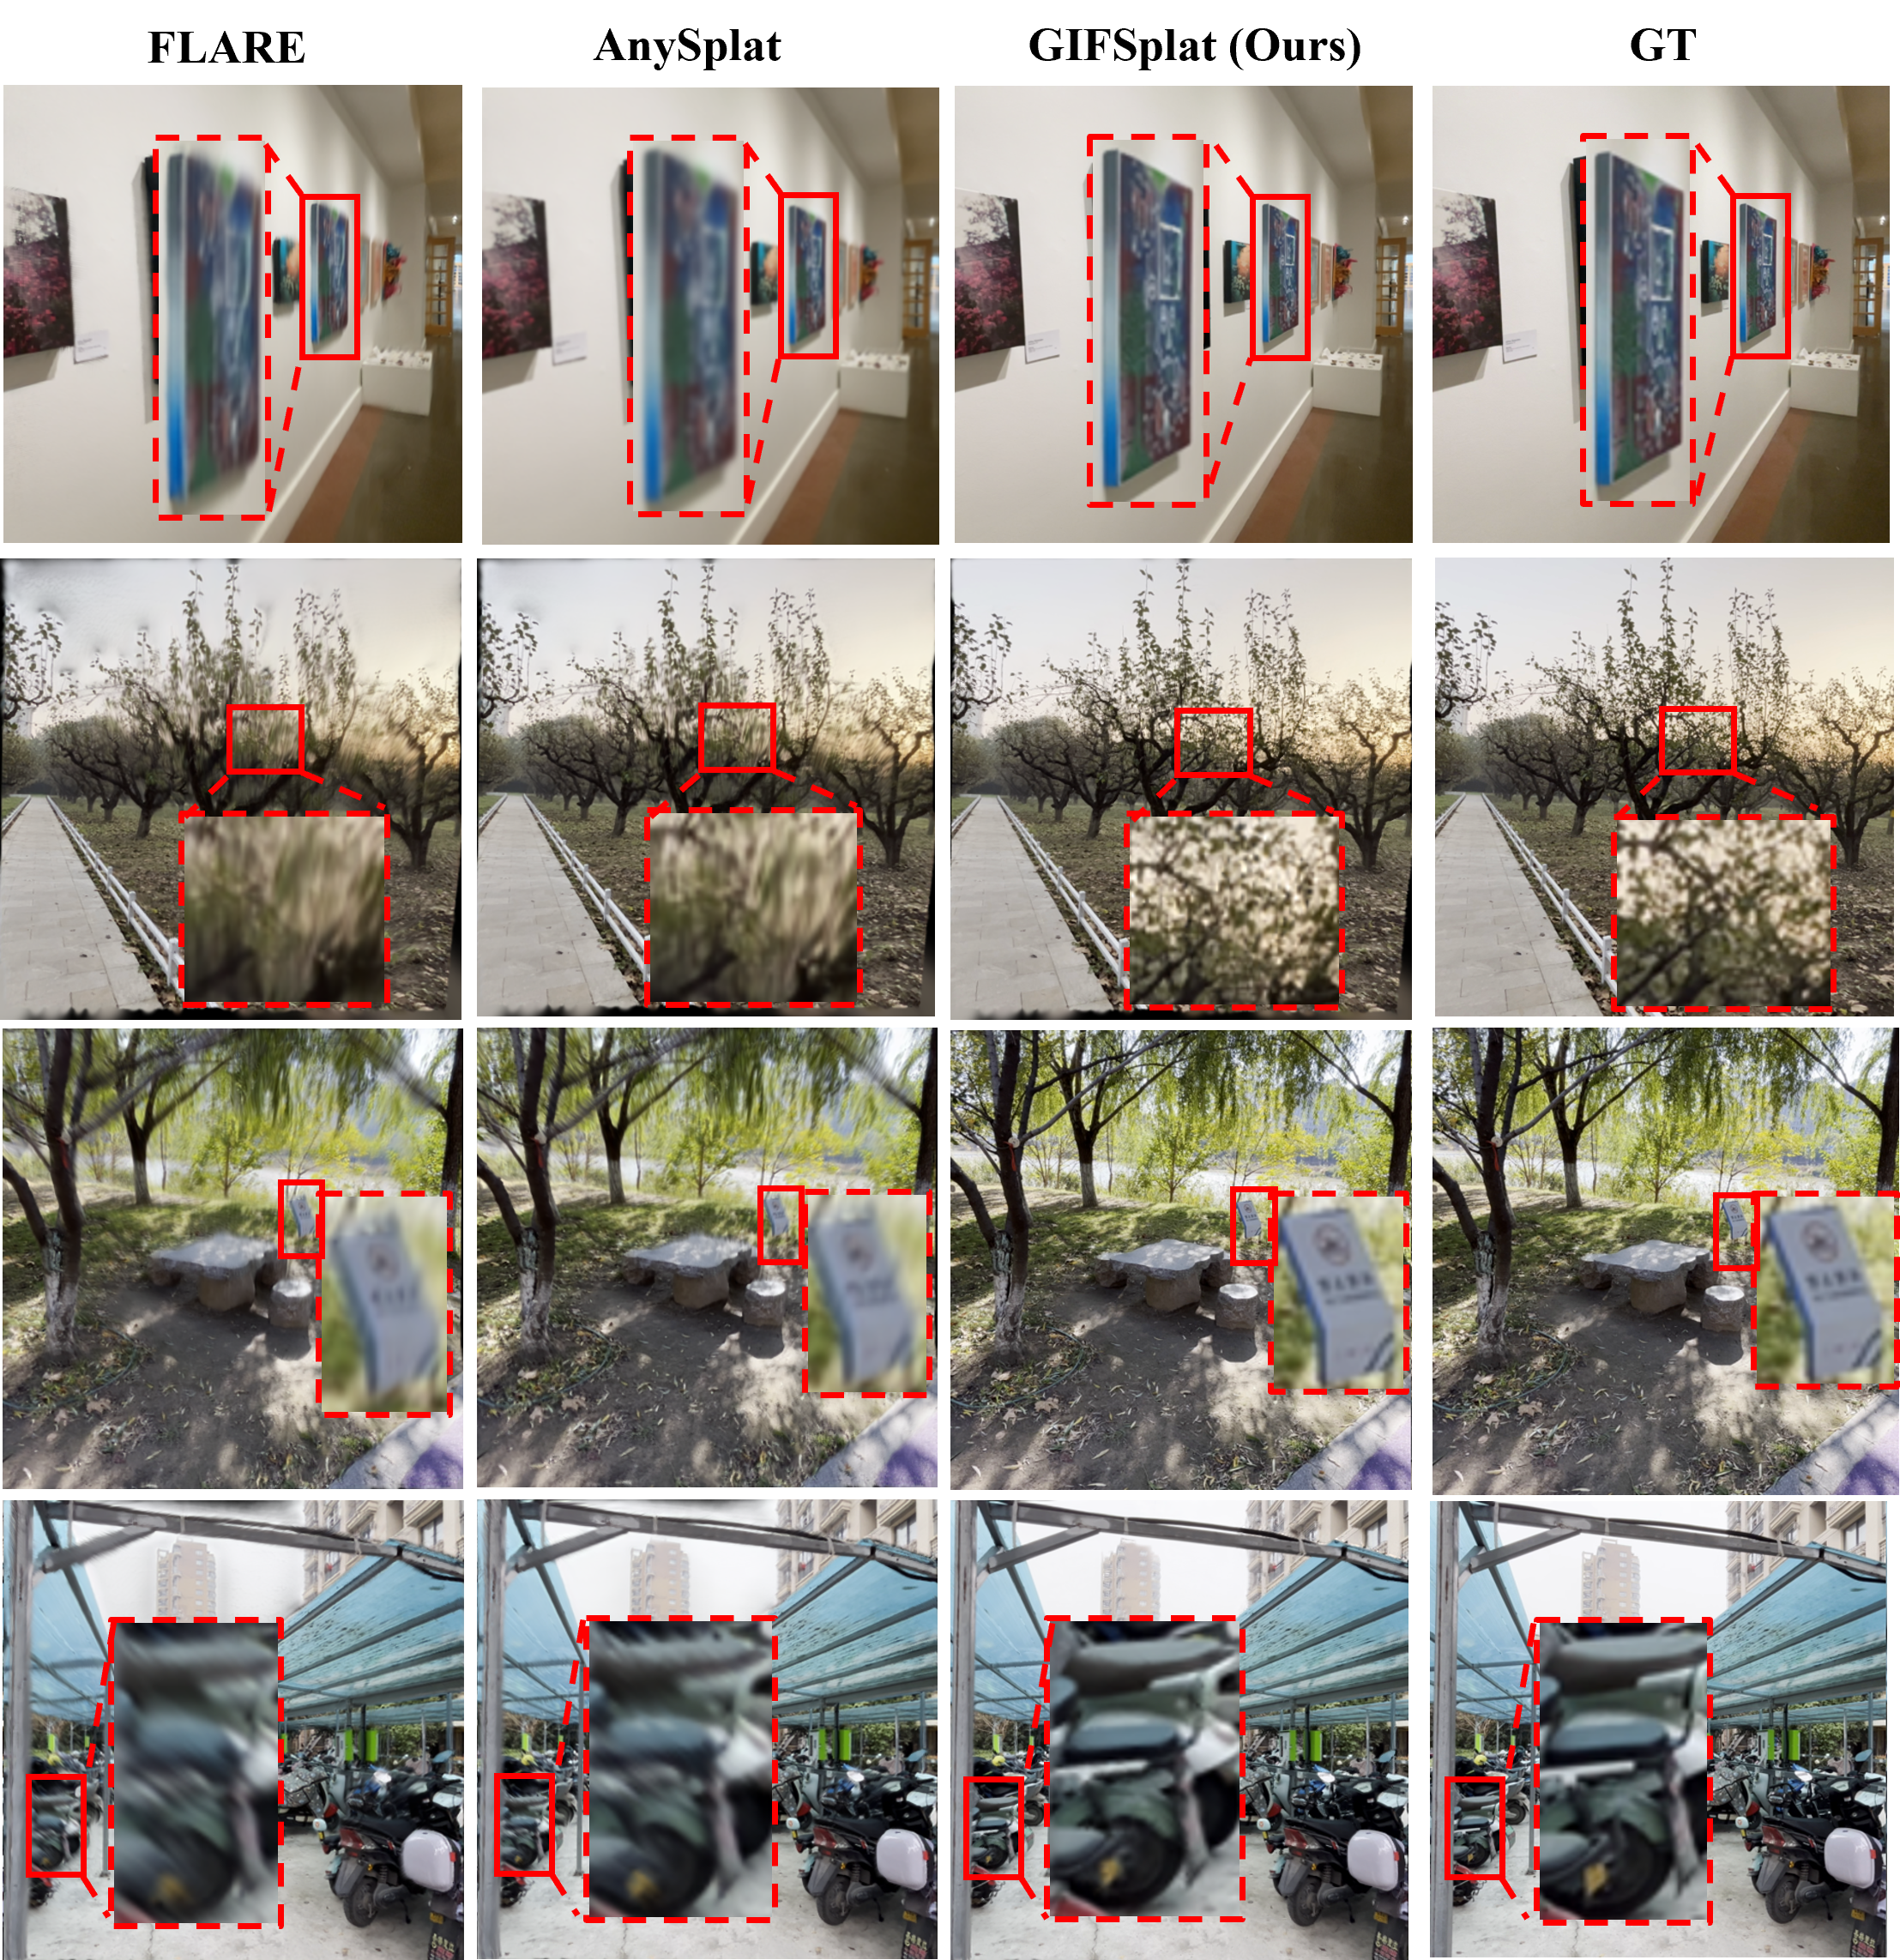
\includegraphics[width=\linewidth]{pics/DL3DV.png}
  \caption{\textbf{Qualitative comparisons on DL3DV}. 
Columns: FLARE, AnySplat, GIFSplat (ours), and GT. 
Across representative scenes, GIFSplat preserves sharper edges and textures while suppressing blur and texture sticking compared with feed-forward baselines. }
\label{fig:DL3DV}
\end{figure}



\paragraph{Generalization to out-of-domain datasets}

~\cref{tab:ood} results of cross-dataset evaluation of baselines, indicate that our iterative residual feed-forward design generalizes well to unconstrained captures, complementing the out-of-domain evaluation on DTU dataset, with over 2 dB performance gain. In addition, we further show the generalization ability of our model in Appendix, demonstrating that the robustness of our model even for in-the-wild images. 

% Preamble:
% \usepackage{booktabs}
% \usepackage{multirow}

% \begin{table}[t]
% \centering
% \caption{\textbf{Out-of-distribution performance comparison}. Our method shows superior performance when zero-shot evaluation on DTU using the model solely trained on RealEstate10K.
% The \textbf{best} and \underline{second-best} results are highlighted.}
% \label{tab:ood}
% \resizebox{0.85\linewidth}{!}{%
% \begin{tabular}{@{}llcccccc@{}}
% \toprule
% \multirow{2}{*}{\textbf{Train}} & \multirow{2}{*}{\textbf{Methods}} & \multicolumn{3}{c}{\textbf{DTU @ 2 views}} \\
% \cmidrule(lr){3-5} 
% & & \textbf{PSNR} $\uparrow$ & \textbf{SSIM} $\uparrow$ & \textbf{LPIPS} $\downarrow$  \\
% \midrule
% \multirow{8}{*}{Real10K} 
% & pixelSplat \cite{charatan2024pixelsplat} & 11.551 & 0.321 & 0.633  \\
% & MVSplat \cite{chen2024mvsplat} & 13.929 & 0.474 & 0.385  \\
% & NopoSplat \cite{ye2024no} & 17.899 & 0.629 & 0.279  \\
% & FLARE \cite{zhang2025flare}  & 17.528 & 0.596 & 0.283  \\
% & AnySplat \cite{jiang2025anysplat} & 18.122 & 0.632 & 0.276  \\
% & \textbf{IFSplat(ours)}    & \underline{19.921} & \underline{0.701} & \underline{0.271}  \\
% & \textbf{GIFSplat(ours)}    & \textbf{20.214} & \textbf{0.712} & \textbf{0.259}  \\
% \bottomrule
% \end{tabular}%
% }
% \end{table}

\begin{table}[t]
\centering
\caption{\textbf{Out-of-distribution performance comparison}. Our method shows superior performance when cross-dataset evaluation on DTU using the model solely trained on RealEstate10K.
The \textbf{best} and \underline{second-best} results are highlighted.}
\label{tab:ood}
\resizebox{0.85\linewidth}{!}{%
\begin{tabular}{@{}lccccccc@{}}
\toprule
\multirow{2}{*}{\textbf{Methods}} & \multirow{2}{*}{\textbf{Pose?}} & \multicolumn{3}{c}{\textbf{DTU @ 2 views}} \\
\cmidrule(lr){3-5} 
& & \textbf{PSNR} $\uparrow$ & \textbf{SSIM} $\uparrow$ & \textbf{LPIPS} $\downarrow$  \\
\midrule
pixelSplat \cite{charatan2024pixelsplat} & \cmark & 11.551 & 0.321 & 0.633  \\
MVSplat \cite{chen2024mvsplat} & \cmark & 13.929 & 0.474 & 0.385  \\
NopoSplat \cite{ye2024no} & \xmark  & 17.899 & 0.629 & 0.279  \\
FLARE \cite{zhang2025flare} & \xmark   & 17.528 & 0.596 & 0.283  \\
AnySplat \cite{jiang2025anysplat} & \xmark  & 18.122 & 0.632 & 0.276  \\
\textbf{IFSplat(ours)}  & \xmark   & \underline{19.921} & \underline{0.701} & \underline{0.274}  \\
\textbf{GIFSplat(ours)}   & \xmark   & \textbf{20.214} & \textbf{0.716} & \textbf{0.251}  \\
\bottomrule
\end{tabular}%
}
\end{table}


\subsection{Ablation Study}
\cref{tab:ablation} validates the contribution of each component. 
Removing the iterative refinement (\emph{\wo Stage~2}) yields the largest degradation across all metrics, confirming the necessity of iterative residual updates.
Disabling the generative prior (\emph{\wo G.~prior}) also reduces performance, particularly in LPIPS, showing that the prior-aware cues effectively suppress artifacts and improve perceptual fidelity.
Disabling the window attention (\emph{\wo window}) also make substantial performance drop, which indicates the function of iteraction in 3D point space.
The full configuration achieves the best performance, demonstrating the complementarity between all components.
\newcolumntype{Y}{>{\raggedright\arraybackslash}p{2.1cm}}
\begin{table}[htbp]
\centering
\footnotesize
\setlength{\tabcolsep}{3pt}
\renewcommand{\arraystretch}{1}
\caption{\textbf{Ablation study. } We ablate the iterative refinement module (\wo Refinement), the window attention (\wo window att.), and the generative prior (\wo Gen. prior) from our full model, respectively. The full configuration achieves the best performance across all metrics.
The \textbf{best} and \underline{second-best} results are highlighted.}
\label{tab:ablation}
\resizebox{.85\columnwidth}{!}{%
\begin{tabular}{Y C{1.3cm} C{1.3cm} C{1.3cm}}
\toprule
\multirow{2}{*}{\textbf{Components}} &
\multicolumn{3}{c}{\textbf{Metrics}} \\
 \cmidrule(lr){2-4} 

& \textbf{PSNR} $\uparrow$ & \textbf{SSIM} $\uparrow$ & \textbf{LPIPS} $\downarrow$ \\
\midrule
\wo Refinement  & 24.781 & 0.826 & 0.169 \\
%\wo feature & & & \\
\wo window att.     & 25.327 & 0.837 & 0.152 \\
\wo Gen. Prior  & \underline{26.291} & \underline{0.854} & \underline{0.145} \\
\textbf{Full} & \textbf{26.559} & \textbf{0.867} & \textbf{0.138}\\
\bottomrule
\end{tabular}}
\end{table}





\subsection{Additional Experiments}
\paragraph{Hyperparameter analysis for iterative steps}
\label{App:hyper}

We vary the number of forward refinements $N$ while keeping all other settings fixed. All experiments are implemented on RealEstate10K dataset in a two-view setting. 
Accuracy improves monotonically from $N{=}0$ and exhibits clear diminishing returns after a few steps. 
%Runtime grows approximately linearly with $N$ because each step performs one rendering and one call to the update head, and the number of Gaussians remains nearly constant across steps. 
In practice we use a small $N=3$ for all main experiments as a favorable trade-off between accuracy and latency .



\begin{table}[htbp]
\centering
\footnotesize
\setlength{\tabcolsep}{3pt}
\renewcommand{\arraystretch}{1}
\caption{\textbf{Analysis of iterative steps.}  We report metrics as the number of refinement steps $T$ increases from the initial prediction, for both IFSplat and our GIFSplat. Performance improves steadily and saturates around 3 iterations.}
\label{tab:ablation}
\resizebox{.95\columnwidth}{!}{%
\begin{tabular}{c C{1.1cm} C{1.1cm} C{1.1cm} C{1.1cm} C{1.1cm} C{1.1cm}}
\toprule
\multirow{2}{*}{\textbf{Steps}} &
\multicolumn{3}{c}{\textbf{Metrics@IFSplat}} & \multicolumn{3}{c}{\textbf{Metrics@GIFSplat}} \\
\cmidrule(lr){2-4}   \cmidrule(lr){5-7} 

& \textbf{PSNR} $\uparrow$ & \textbf{SSIM} $\uparrow$ & \textbf{LPIPS} $\downarrow$ & \textbf{PSNR} $\uparrow$ & \textbf{SSIM} $\uparrow$ & \textbf{LPIPS} $\downarrow$ \\
\midrule
initial  & 24.901 & 0.831 & 0.164 & 24.901 & 0.831 & 0.164  \\
1     & 25.512 & 0.843  &  0.155 & 25.774 & 0.845  &  0.151 \\
2     & 25.873 & 0.847  & 0.150 & 26.107 & 0.849  & 0.147 \\
3     & \underline{26.291} & \underline{0.854} & \textbf{0.145} & \underline{26.559} & \textbf{0.867} & \underline{0.138} \\
4     & \textbf{26.311} & \textbf{0.855} & \textbf{0.146} & \textbf{26.561} & \underline{0.865} & \textbf{0.137} \\

\bottomrule
\end{tabular}}
\end{table}



\paragraph{Additional experiments} 
Due to space constraints, we defer three sets of experiments to the Appendix: (1) a time-complexity analysis of our model, showing that our method retains second-scale runtime even with scene-specific refinement and fusion of generative priors, with Fig.~\ref{fig:time} illustrating one representative part of this analysis; (2) comparisons to 3D reconstruction baselines that incorporate generative priors, demonstrating that our method is consistently superior in both quality and efficiency in sparse-view settings; and (3) experiments on in-the-wild images demonstrating robustness under domain shift. Additional experimental settings, quantitative results, and qualitative visualizations are provided in the Appendix.

\begin{figure}[htbp]
  \centering
  \includegraphics[width=.95\linewidth]{pics/time.pdf}
  \caption{\textbf{Time complexity analysis.} Inference time of our methods IFSplat and GIFSplat on two datasets as a function of the number of refinement steps. Both methods scale approximately linearly with $T$.}%, and GIFSplat introduces a moderate but predictable overhead due to generative prior fusion.}
\label{fig:time}
\end{figure}

% \paragraph{Hyperparameter analysis for iterative steps}
% \label{App:hyper}

% We vary the number of forward refinements $K$ while keeping the view budget per step and all other settings fixed. All experiments are implement on RealEstate10K dataset in 2 view setting.
% Accuracy improves monotonically from $K{=}0$ and exhibits clear diminishing returns after a few steps. 
% Runtime grows approximately linearly with $K$ because each step performs one rendering and one call to the update head, and the number of Gaussians remains nearly constant across steps. 
% In practice we use a small $K$ (e.g., $3$) for all main experiments as a good accuracy/latency trade-off.


% % \begin{table}[htbp]
% % \centering
% % \footnotesize
% % \setlength{\tabcolsep}{3pt}
% % \renewcommand{\arraystretch}{1}
% % \caption{\textbf{Analysis of iterative steps.} We report PSNR, SSIM, LPIPS, and inference time as the number of refinement steps $T$ increases from the initial prediction. Performance steadily improves and largely saturates after about three steps, while the runtime grows roughly linearly with $T$. }
% % \label{tab:ablation}
% % \resizebox{.75\columnwidth}{!}{%
% % \begin{tabular}{c C{1.1cm} C{1.1cm} C{1.1cm} C{1.1cm}}
% % \toprule
% % \multirow{2}{*}{\textbf{Steps}} &
% % \multicolumn{4}{c}{\textbf{Metrics}} \\
% % \cmidrule(lr){2-5} 

% % & \textbf{PSNR} $\uparrow$ & \textbf{SSIM} $\uparrow$ & \textbf{LPIPS} $\downarrow$ & Time $\downarrow$ \\
% % \midrule
% % initial  & 24.901 & 0.831 & 0.164 & 0.15 s  \\
% % 1     & 25.512 & 0.843  &  0.155 & 0.24 s\\
% % 2     & 25.873 & 0.847  & 0.150 & 0.33 s\\
% % 3     & \underline{26.191} & \underline{0.852} & \textbf{0.147} & 0.43 s\\
% % 4     & \textbf{26.212} & \textbf{0.853} & \textbf{0.147} & 0.52 s\\
% % \bottomrule
% % \end{tabular}}
% % \end{table}

% \begin{table}[htbp]
% \centering
% \footnotesize
% \setlength{\tabcolsep}{3pt}
% \renewcommand{\arraystretch}{1}
% \caption{\textbf{Analysis of iterative steps.}  We report PSNR, SSIM, and LPIPS as the number of refinement steps $T$ increases from the initial prediction, for both IFSplat and our GIFSplat. Performance improves steadily and largely saturates after about three steps for all metrics. }
% \label{tab:ablation}
% \resizebox{.95\columnwidth}{!}{%
% \begin{tabular}{c C{1.1cm} C{1.1cm} C{1.1cm} C{1.1cm} C{1.1cm} C{1.1cm}}
% \toprule
% \multirow{2}{*}{\textbf{Steps}} &
% \multicolumn{3}{c}{\textbf{Metrics@IFSplat}} & \multicolumn{3}{c}{\textbf{Metrics@GIFSplat}} \\
% \cmidrule(lr){2-4}   \cmidrule(lr){5-7} 

% & \textbf{PSNR} $\uparrow$ & \textbf{SSIM} $\uparrow$ & \textbf{LPIPS} $\downarrow$ & \textbf{PSNR} $\uparrow$ & \textbf{SSIM} $\uparrow$ & \textbf{LPIPS} $\downarrow$ \\
% \midrule
% initial  & 24.901 & 0.831 & 0.164 & 24.901 & 0.831 & 0.164  \\
% 1     & 25.512 & 0.843  &  0.155 & 25.774 & 0.845  &  0.151 \\
% 2     & 25.873 & 0.847  & 0.150 & 26.107 & 0.849  & 0.147 \\
% 3     & \underline{26.291} & \underline{0.854} & \textbf{0.145} & \underline{26.559} & \textbf{0.867} & \underline{0.138} \\
% 4     & \textbf{26.311} & \textbf{0.855} & \textbf{0.146} & \textbf{26.561} & \underline{0.865} & \textbf{0.137} \\

% \bottomrule
% \end{tabular}}
% \end{table}


% \paragraph{Comparison to 3D reconstruction with generative prior baseline}
% We also compares our feed-forward pipeline with optimization-based approaches DiFiX3D+ and GenFusion under 9-view and 3-view settings. Across both regimes, \textbf{GIFSplat} outperforms substantially and consistently PSNR, SSIM, and LPIPS, while avoiding any test-time optimization and not relying on camera pose. These results indicate that iterative feed-forward updates, coupled with the prior-aware fusion, capture much of the benefit of generative enhancement without incurring the heavy optimization loops.  (see more in Appendix)


% \paragraph{Performance of in-the-wild images}
% To probe robustness beyond curated benchmarks, we evaluate on \emph{in-the-wild} photos. %Whether the input consists of AI-generated videos or real multi-view images, 
% our method consistently infers 3D Gaussian splatting with plausible geometric structures and renders high-quality novel view images. This demonstrates that our model generalizes effectively across diverse input scenarios.(~\cref{fig:wild}).
% The model is trained on DL3DV only and is applied without fine-tuning or camera parameters at test time.
% Across both an indoor tabletop object and a wide-baseline outdoor landscape, GIFSplat generates coherent novel views and faithful textures.

% \begin{figure}[ht]
%   \centering
%   % 在双栏模板中，单栏宽度用 \columnwidth
%   \includegraphics[width=.95\linewidth]{pics/wild.png}
%   \caption{\textbf{In-the-wild qualitative results.}
% Left: handheld phone inputs captured in uncontrolled conditions (auto-exposure, motion, specularities).
% Right: novel-view renderings produced by \textbf{GIFSplat} after a few forward-only residual updates, without using camera intrinsics/extrinsics.
% Our reconstructions preserve edges and textures while maintaining multi-view consistency across challenging indoor and outdoor scenes.
% Zoom in for details.}
%   \label{fig:wild}
% \end{figure}




% TODO list
% 1. adding per example PSNR metirc in figure
% 2. rewrite section experiments, make it clear. Most importantly, give some insights and analysis rather than directly describe the result (it like a experiments report rather than scientific paper)


